\subsection{Evaluation}

In order to evaluate the performance of our queries we compare a manually selected list of relevant documents with the ones returned by the system. To assess the improvements provided by our schema, we compared it to a simpler counterpart, using only lower case filters. The metrics utilized to compare our schema to the simpler one are a \textbf{Precision-Recall Curve}, the average precision and precision at 10, which are described below.


\begin{itemize}
    \item Average Precision (AP): The average of the precision values obtained for the set of top N documents existing each time a new relevant document is retrieved.
    \item Precision at 10 (P@10): Precision at a specific cut point in the result ranked list, in this case 10, i.e. the ratio of the first 10 values that are relevant.
    \item Precision-Recall Curve: A graph that illustrates how precision varies according to recall, providing insights into how the system performs at varying degrees of scrutiny.

\end{itemize}

\textbf{Query 1}

Below are present the evaluation result's for the simpler schema:

\begin{center}
\begin{tabular}{lll}
\toprule
 &                  Metric &    Value \\
\midrule
1 &       Average Precision &  0.817857 \\
2 &  Precision at 10 (P@10) &      0.6 \\
\bottomrule
\end{tabular}
\end{center}

\begin{figure}[H]
    \centering
    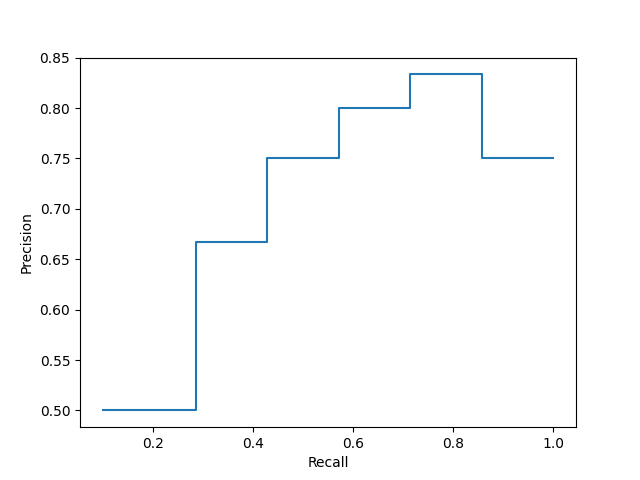
\includegraphics[width=0.6\linewidth]{figures/toxic_simple.png}
    \caption{Simple schema's Precision-Recall Curve}
\end{figure}

As we can see below, the boosting had a noticeable effect on the performance of our system:

\begin{center}
\begin{tabular}{lll}
\toprule
 &                  Metric &    Value \\
\midrule
1 &       Average Precision &  0.97619 \\
2 &  Precision at 10 (P@10) &      0.6 \\
\bottomrule
\end{tabular}
\end{center}

\begin{figure}[H]
    \centering
    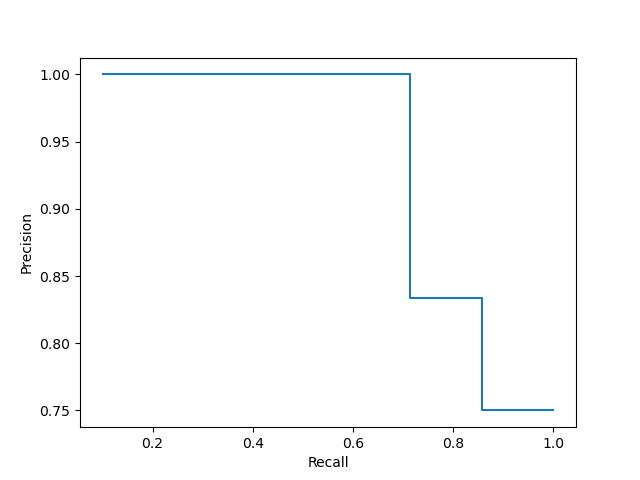
\includegraphics[width=0.6\linewidth]{figures/toxic.png}
    \caption{Refined schema's Precision-Recall Curve}
\end{figure}



\textbf{Query 2}

Again, below are presented the performance results for the simpler schema:

\begin{center}
\begin{tabular}{lll}
\toprule
 &                  Metric &    Value \\
\midrule
1 &       Average Precision &  0.877381 \\
2 &  Precision at 10 (P@10) &       0.6 \\
\bottomrule
\end{tabular}
\end{center}

\begin{figure}[H]
    \centering
    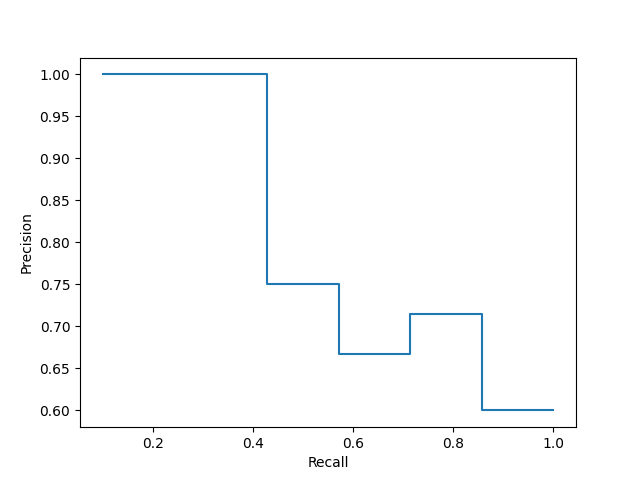
\includegraphics[width=0.6\linewidth]{figures/disease_simple.png}
    \caption{Simple schema's Precision-Recall Curve}
\end{figure}

Finally, the performance results for the refined schema:

\begin{center}
\begin{tabular}{lll}
\toprule
 &                  Metric &    Value \\
\midrule
1 &       Average Precision &  0.930556 \\
2 &  Precision at 10 (P@10) &       0.6 \\
\bottomrule
\end{tabular}
\end{center}

\begin{figure}[H]
    \centering
    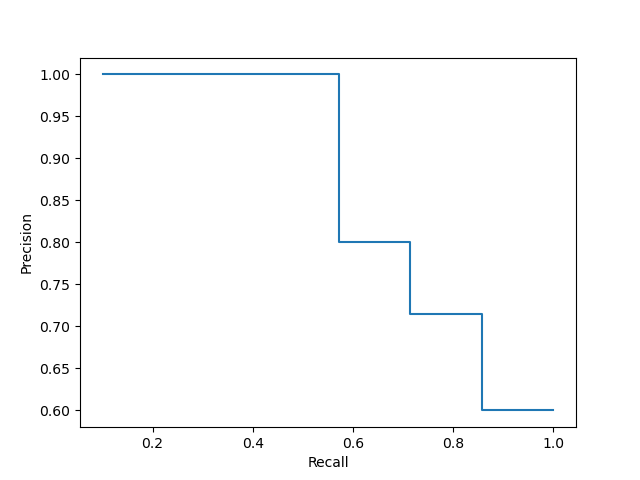
\includegraphics[width=0.6\linewidth]{figures/disease.png}
    \caption{Refined schema's Precision-Recall Curve}
\end{figure}





